\documentclass[11pt,a4paper]{report}
\usepackage[textwidth=37em,vmargin=30mm]{geometry}
\usepackage{calc,xunicode,amsmath,amssymb,paralist,enumitem,tabu,booktabs,datetime2,xeCJK,xeCJKfntef,listings}
\usepackage{tocloft,fancyhdr,tcolorbox,xcolor,graphicx,eso-pic,xltxtra,xelatexemoji}

\newcommand{\envyear}[0]{2025}
\newcommand{\envdatestr}[0]{2025-03-05}
\newcommand{\envfinaldir}[0]{webdb/2025/20250305/final}

\usepackage[hidelinks]{hyperref}
\hypersetup{
    colorlinks=false,
    pdfpagemode=FullScreen,
    pdftitle={Web Digest - \envdatestr}
}

\setlength{\cftbeforechapskip}{10pt}
\renewcommand{\cftchapfont}{\rmfamily\bfseries\large\raggedright}
\setlength{\cftbeforesecskip}{2pt}
\renewcommand{\cftsecfont}{\sffamily\small\raggedright}

\setdefaultleftmargin{2em}{2em}{1em}{1em}{1em}{1em}

\usepackage{xeCJK,xeCJKfntef}
\xeCJKsetup{PunctStyle=plain,RubberPunctSkip=false,CJKglue=\strut\hskip 0pt plus 0.1em minus 0.05em,CJKecglue=\strut\hskip 0.22em plus 0.2em}
\XeTeXlinebreaklocale "zh"
\XeTeXlinebreakskip = 0pt


\setmainfont{Brygada 1918}
\setromanfont{Brygada 1918}
\setsansfont{IBM Plex Sans}
\setmonofont{JetBrains Mono NL}
\setCJKmainfont{Noto Serif CJK SC}
\setCJKromanfont{Noto Serif CJK SC}
\setCJKsansfont{Noto Sans CJK SC}
\setCJKmonofont{Noto Sans CJK SC}

\setlength{\parindent}{0pt}
\setlength{\parskip}{8pt}
\linespread{1.15}

\lstset{
	basicstyle=\ttfamily\footnotesize,
	numbersep=5pt,
	backgroundcolor=\color{black!5},
	showspaces=false,
	showstringspaces=false,
	showtabs=false,
	tabsize=2,
	captionpos=b,
	breaklines=true,
	breakatwhitespace=true,
	breakautoindent=true,
	linewidth=\textwidth
}






\newcommand{\coverpic}[2]{
    % argv: itemurl, authorname
    Cover photo by #2~~(\href{#1}{#1})
}
\newcommand{\makeheader}[0]{
    \begin{titlepage}
        % \newgeometry{hmargin=15mm,tmargin=21mm,bmargin=12mm}
        \begin{center}
            
            \rmfamily\scshape
            \fontspec{BaskervilleF}
            \fontspec{Old Standard}
            \fontsize{59pt}{70pt}\selectfont
            WEB\hfill DIGEST
            
            \vfill
            % \vskip 30pt
            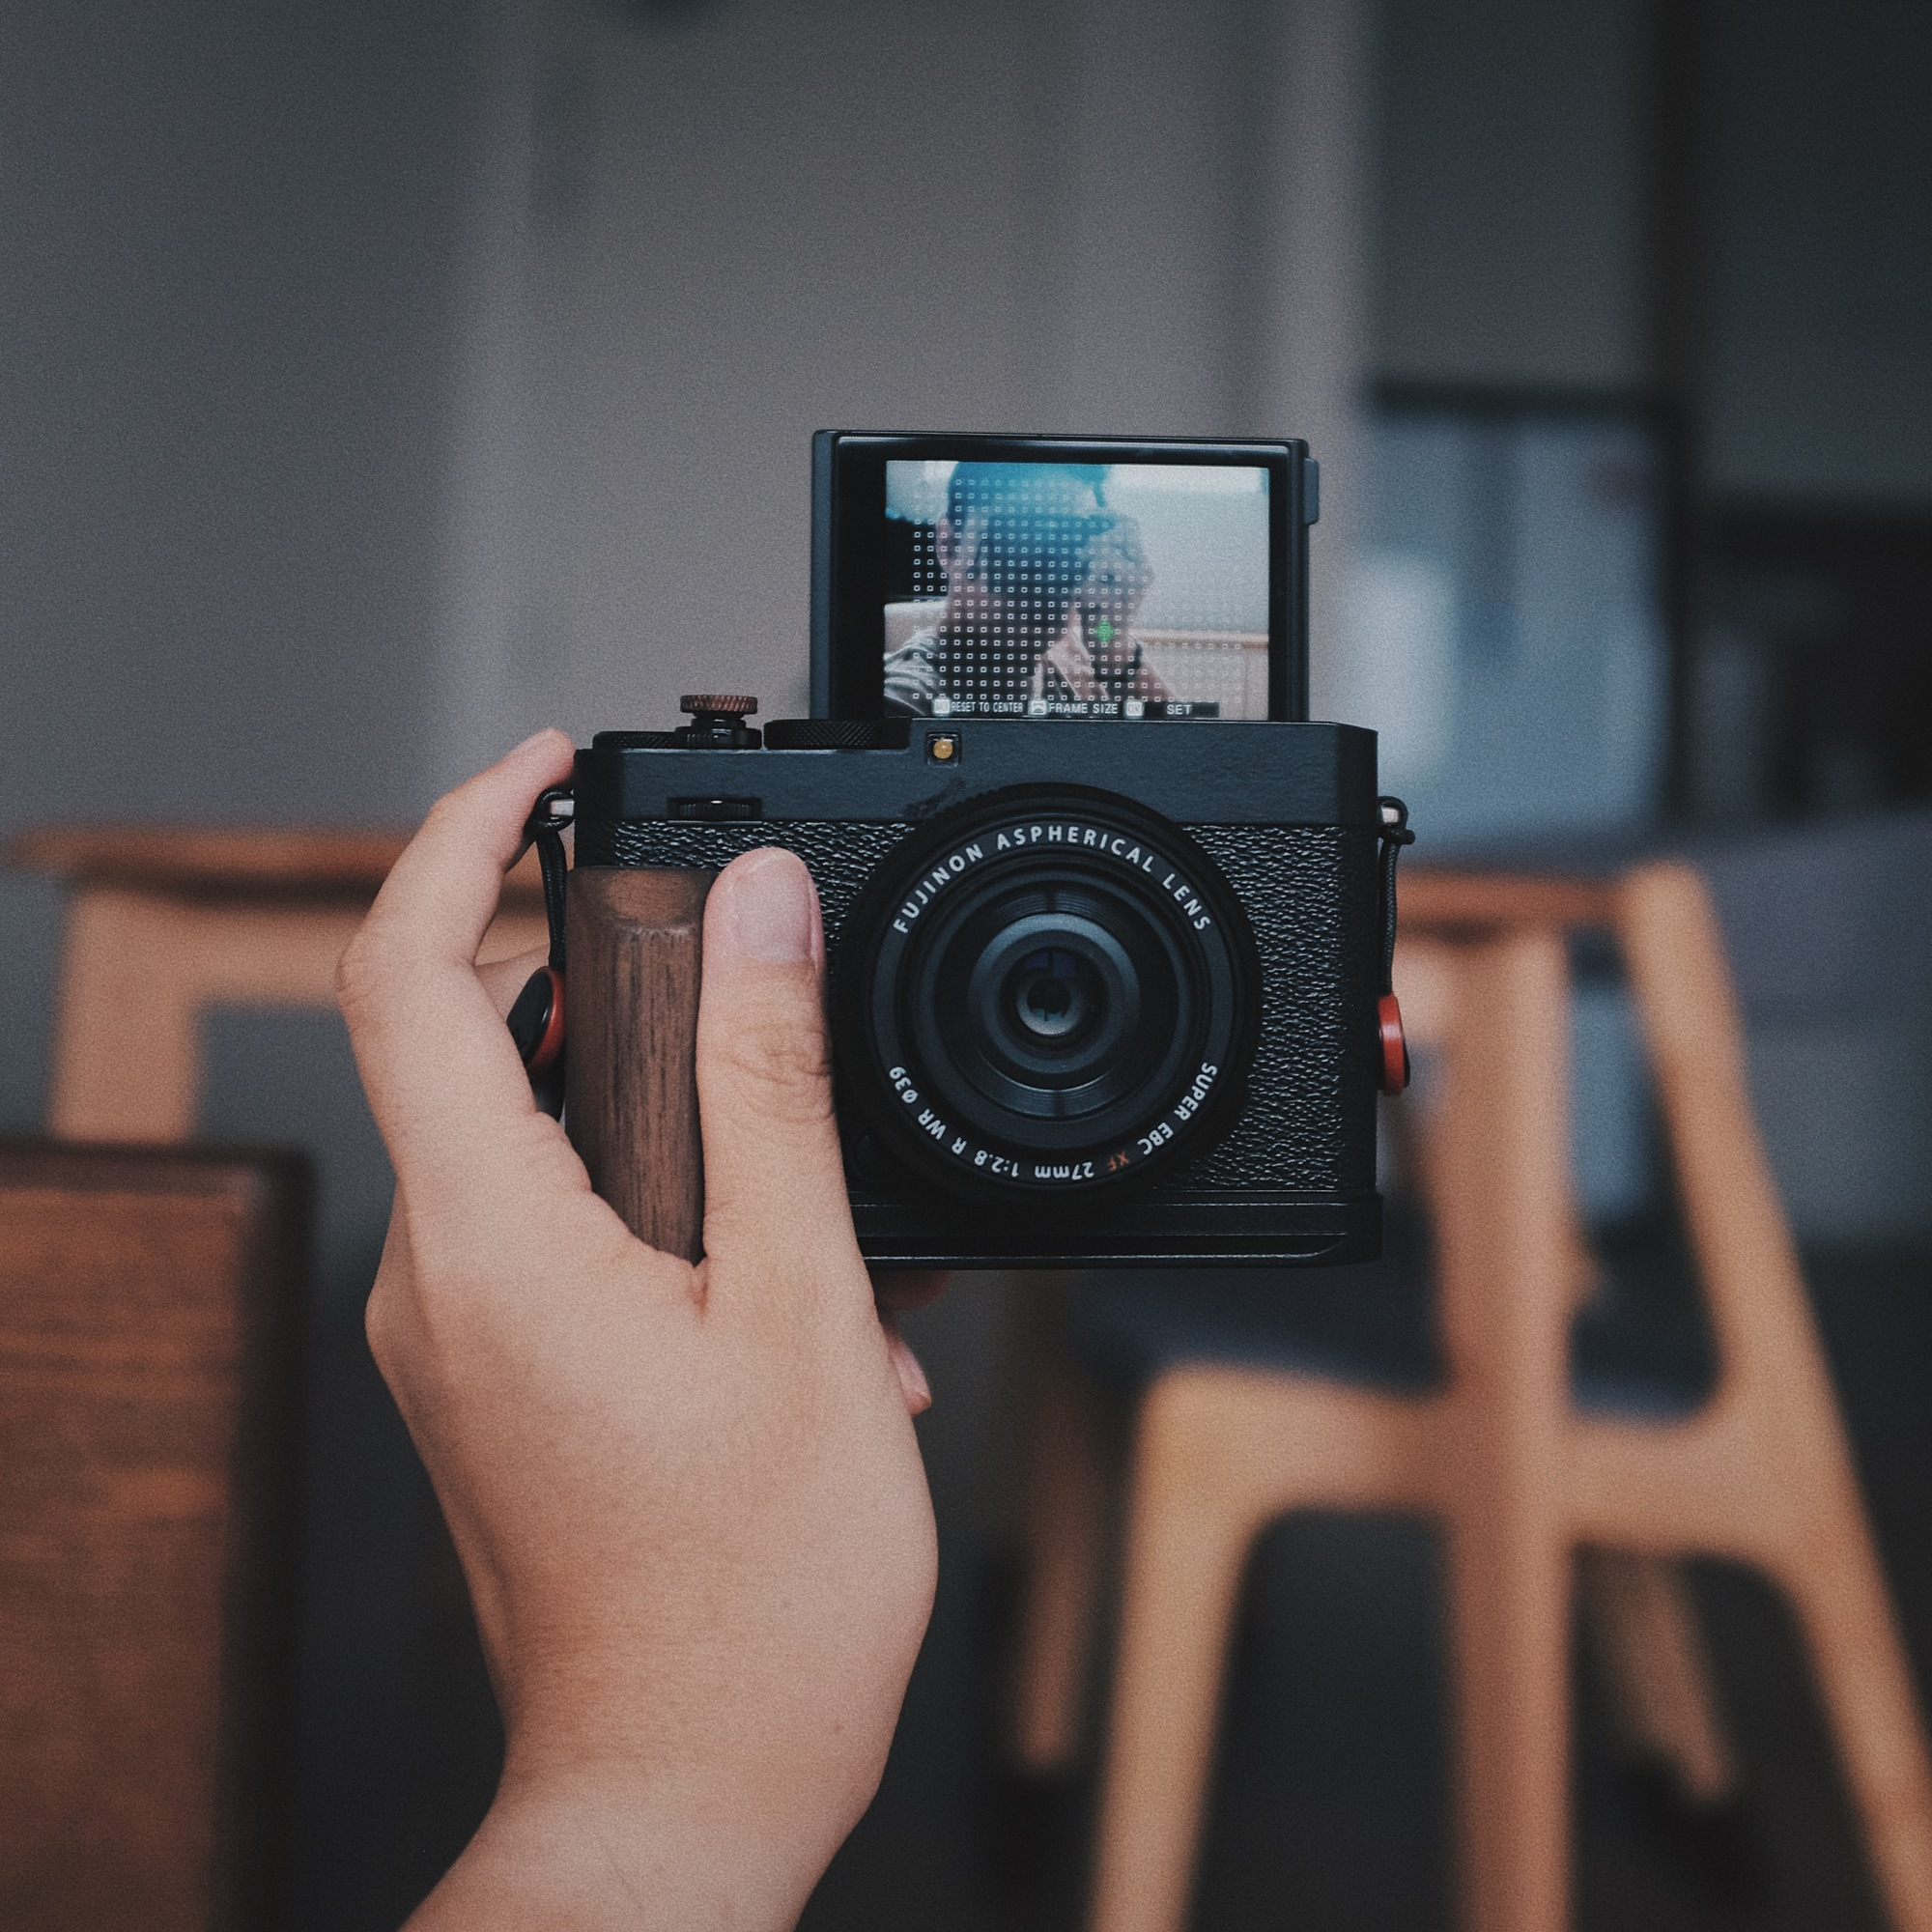
\includegraphics[width=\linewidth]{\envfinaldir/coverpic-prod.jpg}\par
            % \vskip 30pt
            \vfill

            \normalsize\rmfamily\scshape
            \copyright{} The Web Digest Project \hfill\large \envdatestr
        \end{center}
    \end{titlepage}
    % \restoregeometry
}
\newcommand{\simplehref}[1]{%
    \textcolor{blue!80!green}{\href{#1}{#1}}%
}
\renewcommand{\contentsname}{\center\Huge\sffamily\bfseries Contents\par\vskip 20pt}
\newcounter{ipartcounter}
\setcounter{ipartcounter}{0}
\newcommand{\ipart}[1]{
    % \vskip 20pt
    \clearpage
    \stepcounter{ipartcounter}
    \phantomsection
    \addcontentsline{toc}{chapter}{#1}
    % \begin{center}
    %     \Huge
    %     \sffamily\bfseries
    %     #1
    % \end{center}
    % \vskip 20pt plus 7pt
}
\newcounter{ichaptercounter}
\setcounter{ichaptercounter}{0}
\newcommand{\ichapter}[1]{
    % \vskip 20pt
    \clearpage
    \stepcounter{ichaptercounter}
    \phantomsection
    \addcontentsline{toc}{section}{\numberline{\arabic{ichaptercounter}}#1}
    \begin{center}
        \Huge
        \sffamily\bfseries
        #1
    \end{center}
    \vskip 20pt plus 7pt
}
\newcommand{\entrytitlefont}[1]{\subsection*{\raggedright\Large\sffamily\bfseries#1}}
\newcommand{\entryitemGeneric}[2]{
    % argv: title, url
    \parbox{\linewidth}{
        \entrytitlefont{#1}\par\vskip 5pt
        \footnotesize\ttfamily\mdseries
        \simplehref{#2}
    }\vskip 11pt plus 11pt minus 1pt
}
\newcommand{\entryitemGithub}[3]{
    % argv: title, url, desc
    \parbox{\linewidth}{
        \entrytitlefont{#1}\par\vskip 5pt
        \footnotesize\ttfamily\mdseries
        \simplehref{#2}\par\vskip 5pt
        \small\rmfamily\mdseries#3
    }\vskip 11pt plus 11pt minus 1pt
}
\newcommand{\entryitemAp}[3]{
    % argv: title, url, desc
    \parbox{\linewidth}{
        \entrytitlefont{#1}\par\vskip 5pt
        \footnotesize\ttfamily\mdseries
        \simplehref{#2}\par\vskip 5pt
        \small\rmfamily\mdseries#3
    }\vskip 11pt plus 11pt minus 1pt
}
\newcommand{\entryitemHackernews}[3]{
    % argv: title, hnurl, rawurl
    % \parbox{\linewidth}{
    %     \entrytitlefont{#1}\par\vskip 5pt
    %     \footnotesize\ttfamily\mdseries
    %     \simplehref{#3}\par
    %     \textcolor{black!50}{\href{#2}{#2}}
    % }\vskip 11pt plus 11pt minus 1pt
    \begin{minipage}{\linewidth}
            \entrytitlefont{#1}\par\vskip 5pt
            \footnotesize\ttfamily\mdseries
            \simplehref{#3}\par
            \textcolor{black!50}{\href{#2}{#2}}
    \end{minipage}\par\vskip 11pt plus 11pt minus 1pt
}







\begin{document}

\makeheader

\tableofcontents\clearpage




\ipart{Developers}
\ichapter{Hacker News}
\entryitemTwoLinks{ARC-AGI without pretraining}{https://news.ycombinator.com/item?id=43259182}{https://iliao2345.github.io/blog\_posts/arc\_agi\_without\_pretraining/arc\_agi\_without\_pretraining.html}

\entryitemTwoLinks{Why fastDOOM is fast}{https://news.ycombinator.com/item?id=43258709}{https://fabiensanglard.net/fastdoom/index.html}

\entryitemTwoLinks{Translating natural language to first-order logic for logical fallacy detection}{https://news.ycombinator.com/item?id=43257719}{https://arxiv.org/abs/2405.02318}

\entryitemTwoLinks{Learn How to Break AES}{https://news.ycombinator.com/item?id=43257583}{https://davidwong.fr/blockbreakers/}

\entryitemTwoLinks{Satellogic's Open Satellite Feed}{https://news.ycombinator.com/item?id=43256349}{https://tech.marksblogg.com/satellogic-open-data-feed.html}

\entryitemTwoLinks{The owner of ip4.me/ip6.me, Kevin Loch, has died}{https://news.ycombinator.com/item?id=43256298}{https://ip4only.me/}

\entryitemTwoLinks{Show HN: Bayleaf – Building a low-profile wireless split keyboard}{https://news.ycombinator.com/item?id=43255529}{https://www.graz.io/articles/bayleaf-wireless-keyboard}

\entryitemTwoLinks{DIY "infinity contrast" TV – with 100\% recycled parts [video]}{https://news.ycombinator.com/item?id=43255446}{https://www.youtube.com/watch?v=qXrn4MqY1Wo}

\entryitemTwoLinks{Federal workers ordered to return to offices without desks, Wi-Fi and lights}{https://news.ycombinator.com/item?id=43253562}{https://www.cnn.com/2025/03/04/politics/federal-employees-return-to-office-problems/index.html}

\entryitemTwoLinks{Italy moves to reverse anti-nuclear stance}{https://news.ycombinator.com/item?id=43253407}{https://www.world-nuclear-news.org/articles/cabinet-moves-to-reverse-italys-anti-nuclear-stance}

\entryitemTwoLinks{The End of Weather Forecasting}{https://news.ycombinator.com/item?id=43251150}{https://thinc.blog/2025/03/03/the-end-of-weather-forecasting/}

\entryitemTwoLinks{Let's code a TCP/IP stack, 1: Ethernet and ARP (2016)}{https://news.ycombinator.com/item?id=43250093}{https://www.saminiir.com/lets-code-tcp-ip-stack-1-ethernet-arp/}

\entryitemTwoLinks{Global sales of combustion engine cars have peaked}{https://news.ycombinator.com/item?id=43249068}{https://ourworldindata.org/data-insights/global-sales-of-combustion-engine-cars-have-peaked}

\entryitemTwoLinks{DeepSeek's smallpond: Bringing Distributed Computing to DuckDB}{https://news.ycombinator.com/item?id=43248947}{https://mehdio.substack.com/p/duckdb-goes-distributed-deepseeks}

\entryitemTwoLinks{U.S. pauses all military aid to Ukraine}{https://news.ycombinator.com/item?id=43248919}{https://www.wsj.com/politics/national-security/u-s-hitting-brakes-on-flow-of-arms-to-ukraine-980a71d1}

\entryitemTwoLinks{Public health data disappeared. RestoredCDC.org is bringing it back}{https://news.ycombinator.com/item?id=43248610}{https://www.RestoredCDC.org}

\entryitemTwoLinks{Lawrence of Arabia, Paul Atreides, and the roots of Frank Herbert's Dune (2021)}{https://news.ycombinator.com/item?id=43248429}{https://reactormag.com/lawrence-of-arabia-paul-atreides-and-the-roots-of-frank-herberts-dune/}

\entryitemTwoLinks{Repairable Flatpack Toaster}{https://news.ycombinator.com/item?id=43246892}{https://www.kaseyhou.com/\#/repairable-flatpack-toaster/}

\entryitemTwoLinks{Comparing Fuchsia components and Linux containers [video]}{https://news.ycombinator.com/item?id=43246703}{https://fosdem.org/2025/schedule/event/fosdem-2025-5381-comparing-fuchsia-components-and-linux-containers/}

\entryitemTwoLinks{Atlanta Fed predicts -2.8\% GDP}{https://news.ycombinator.com/item?id=43246371}{https://www.atlantafed.org/cqer/research/gdpnow}\ichapter{Phoronix}
\entryitemGeneric{\hskip 0pt{}AMD ZenDNN 5.0.1 Released To Help With EPYC Inferencing For Recommender Systems \& LLMs}{https://www.phoronix.com/news/AMD-ZenDNN-5.0.1}

\entryitemGeneric{\hskip 0pt{}LLVM/Clang 20.1 Released With AMX-AVX512, AMX-FP8, AVX10.2, AMD GFX950 \& Much More}{https://www.phoronix.com/news/LLVM-20.1-Released}

\entryitemGeneric{\hskip 0pt{}Firefox 137 Beta Now Available With VA-API Accelerated H.265/HEVC On Linux}{https://www.phoronix.com/news/Firefox-137-Beta-Released}

\entryitemGeneric{\hskip 0pt{}Intel Finds More Women Getting Involved In Open-Source, Maintainer Burnout Continues}{https://www.phoronix.com/news/Intel-Open-Source-Survey-2024}

\entryitemGeneric{\hskip 0pt{}ExpressVPN Adds A GUI To Their Linux App}{https://www.phoronix.com/news/ExpressVPN-GUI-Linux-App}

\entryitemGeneric{\hskip 0pt{}NVIDIA GeForce RTX 5070 Linux GPU Compute Performance}{https://www.phoronix.com/review/nvidia-rtx-5070-linux}

\entryitemGeneric{\hskip 0pt{}Perforator 0.0.5 Released - Switches To Apache 2.0 License, Drops CLA Requirement}{https://www.phoronix.com/news/Yandex-Perforator-0.0.5}

\entryitemGeneric{\hskip 0pt{}Linux's AMD Radeon Vulkan Driver Adds Experimental Support For The BC-250 Mining Board}{https://www.phoronix.com/news/Mesa-25.1-RADV-AMD-BC-250}

\entryitemGeneric{\hskip 0pt{}Direct3D Video Decode To Vulkan Video API Being Worked On For Wine}{https://www.phoronix.com/news/Wine-Direct3D-Video-To-Vulkan}\ichapter{Dribbble}
\entryitemGeneric{\hskip 0pt{}Star + Check Mark Icon Concept}{https://dribbble.com/shots/25709690-Star-Check-Mark-Icon-Concept}

\entryitemGeneric{\hskip 0pt{}FREELANCE (Finally)}{https://dribbble.com/shots/25710537-FREELANCE-Finally}

\entryitemGeneric{\hskip 0pt{}Recent Logo Designs - Jeroen van Eerden}{https://dribbble.com/shots/25709914-Recent-Logo-Designs-Jeroen-van-Eerden}

\entryitemGeneric{\hskip 0pt{}Wolf}{https://dribbble.com/shots/25707625-Wolf}

\entryitemGeneric{\hskip 0pt{}Star + Check Mark Icon Concept}{https://dribbble.com/shots/25698016-Star-Check-Mark-Icon-Concept}

\entryitemGeneric{\hskip 0pt{}Block13 Promo Board Design /1 /2 /3}{https://dribbble.com/shots/25700177-Block13-Promo-Board-Design-1-2-3}

\entryitemGeneric{\hskip 0pt{}Communication Illustration}{https://dribbble.com/shots/25700541-Communication-Illustration}

\entryitemGeneric{\hskip 0pt{}Tally Logo Design}{https://dribbble.com/shots/25693309-Tally-Logo-Design}

\entryitemGeneric{\hskip 0pt{}Letter A}{https://dribbble.com/shots/25691267-Letter-A}

\entryitemGeneric{\hskip 0pt{}Detective Dog Logo}{https://dribbble.com/shots/25692587-Detective-Dog-Logo}

\entryitemGeneric{\hskip 0pt{}HyperSeed - Logo Design}{https://dribbble.com/shots/25692269-HyperSeed-Logo-Design}

\entryitemGeneric{\hskip 0pt{}Logo Design for Gaming Platform (Unused for Sale)}{https://dribbble.com/shots/25692257-Logo-Design-for-Gaming-Platform-Unused-for-Sale}

\entryitemGeneric{\hskip 0pt{}Barbershop app dashboard}{https://dribbble.com/shots/25687859-Barbershop-app-dashboard}

\entryitemGeneric{\hskip 0pt{}NonStop}{https://dribbble.com/shots/25692105-NonStop}

\entryitemGeneric{\hskip 0pt{}Jiggy's Court™}{https://dribbble.com/shots/25693857-Jiggy-s-Court}

\entryitemGeneric{\hskip 0pt{}Finance app ui Design}{https://dribbble.com/shots/25691020-Finance-app-ui-Design}

\entryitemGeneric{\hskip 0pt{}—From Archive (Pt. 10)}{https://dribbble.com/shots/25692986--From-Archive-Pt-10}

\entryitemGeneric{\hskip 0pt{}Ramotion Logo Design}{https://dribbble.com/shots/25582478-Ramotion-Logo-Design}

\entryitemGeneric{\hskip 0pt{}Cimet Stationery}{https://dribbble.com/shots/25687823-Cimet-Stationery}

\entryitemGeneric{\hskip 0pt{}Check Mark App Icon}{https://dribbble.com/shots/25687869-Check-Mark-App-Icon}

\entryitemGeneric{\hskip 0pt{}Block13 Promo Board Design}{https://dribbble.com/shots/25688403-Block13-Promo-Board-Design}

\entryitemGeneric{\hskip 0pt{}Vitra - Logo Design}{https://dribbble.com/shots/25686757-Vitra-Logo-Design}

\entryitemGeneric{\hskip 0pt{}Bowls \& Blasters}{https://dribbble.com/shots/25687511-Bowls-Blasters}

\entryitemGeneric{\hskip 0pt{}Apparel design for Carhartt 03}{https://dribbble.com/shots/25689259-Apparel-design-for-Carhartt-03}


\ipart{Developers~~~~(zh-Hans)}
\ichapter{Solidot}
\entryitemGeneric{\hskip 0pt{}AI 娱乐公司以模因币竞标 Infowars}{https://www.solidot.org/story?sid=80706}

\entryitemGeneric{\hskip 0pt{}火星的红色可能来自水铁矿}{https://www.solidot.org/story?sid=80705}

\entryitemGeneric{\hskip 0pt{}拯救了 240 万婴儿的澳大利亚人 James Harrison 去世}{https://www.solidot.org/story?sid=80704}

\entryitemGeneric{\hskip 0pt{}欧洲刑警组织逮捕 25 名分享 AI 儿童色情的用户}{https://www.solidot.org/story?sid=80703}

\entryitemGeneric{\hskip 0pt{}芹菜西兰花中的天然成分能抑制白发}{https://www.solidot.org/story?sid=80702}

\entryitemGeneric{\hskip 0pt{}美国将设加密货币战略储备}{https://www.solidot.org/story?sid=80701}

\entryitemGeneric{\hskip 0pt{}新方头鱼物种以《幽灵公主》角色命名}{https://www.solidot.org/story?sid=80700}

\entryitemGeneric{\hskip 0pt{}科学家发现人类祖先在 15 万年前生活在非洲雨林的证据}{https://www.solidot.org/story?sid=80699}

\entryitemGeneric{\hskip 0pt{}卡巴斯基在 GitHub 上发现隐藏的恶意程序}{https://www.solidot.org/story?sid=80698}

\entryitemGeneric{\hskip 0pt{}Firefly `Blue Ghost' 成功登陆月球表面}{https://www.solidot.org/story?sid=80697}

\entryitemGeneric{\hskip 0pt{}用 Blender 制作的《Flow》赢得奥斯卡最佳动画片}{https://www.solidot.org/story?sid=80696}

\entryitemGeneric{\hskip 0pt{}哈工大研发可用于火星的空地两用无人机}{https://www.solidot.org/story?sid=80695}

\entryitemGeneric{\hskip 0pt{}tzram-audit: ARM TrustZone内存隔离审计}{https://www.solidot.org/story?sid=80694}

\entryitemGeneric{\hskip 0pt{}创业公司延长狗命的药物获得 FDA 的初步认可}{https://www.solidot.org/story?sid=80693}

\entryitemGeneric{\hskip 0pt{}Microsoft Azure 彻底禁止域前置,影响 Tor Browser 内置网桥}{https://www.solidot.org/story?sid=80692}

\entryitemGeneric{\hskip 0pt{}犹他州有望成为美国第一个在公共自来水中禁用氟的州}{https://www.solidot.org/story?sid=80691}\ichapter{V2EX}
\entryitemGeneric{\hskip 0pt{}[分享创造] 专为公众号引用链接设计,一行代码没写用 ai 开发了一个链接转图片的网站}{https://www.v2ex.com/t/1115942}

\entryitemGeneric{\hskip 0pt{}[问与答] 字节国内版的 Trae 发布了,大家觉得好用吗?跟国外版本的 Trae 差别大吗?}{https://www.v2ex.com/t/1115941}

\entryitemGeneric{\hskip 0pt{}[5G] 求推荐:移动量大管饱的流量套餐}{https://www.v2ex.com/t/1115940}

\entryitemGeneric{\hskip 0pt{}[旅行] 这个社区对「潜水」感兴趣的人多吗}{https://www.v2ex.com/t/1115938}

\entryitemGeneric{\hskip 0pt{}[问与答] 关于 BIOS 上的一条提示信息 Verifying DMI Pool Data …… 寻求相关帮助}{https://www.v2ex.com/t/1115937}

\entryitemGeneric{\hskip 0pt{}[生活] 一年半前发帖准备移居,如今落地温哥华两周了,谈谈感想}{https://www.v2ex.com/t/1115936}

\entryitemGeneric{\hskip 0pt{}[分享发现] 🎯Insightly.top 来啦!智能分析用户评论,秒得关键反馈!}{https://www.v2ex.com/t/1115935}

\entryitemGeneric{\hskip 0pt{}[旅行] 4 月 2-16 去日本旅游,有什么推荐/叮嘱?}{https://www.v2ex.com/t/1115933}

\entryitemGeneric{\hskip 0pt{}[YouTube] 弱弱问一句,为什么我的频道没有播放量?}{https://www.v2ex.com/t/1115932}

\entryitemGeneric{\hskip 0pt{}[Apple] Mac mini m4 重启后无法连接安克 usb hub}{https://www.v2ex.com/t/1115931}

\entryitemGeneric{\hskip 0pt{}[Chrome] chrome 插件问题}{https://www.v2ex.com/t/1115929}

\entryitemGeneric{\hskip 0pt{}[Apple] mac 外接硬盘能否开启 AI}{https://www.v2ex.com/t/1115928}

\entryitemGeneric{\hskip 0pt{}[程序员] vscode(cursor)的 cmake tools 运行按钮为什么点了没反应?}{https://www.v2ex.com/t/1115927}

\entryitemGeneric{\hskip 0pt{}[程序员] 国内的网站 ban 国外 ip 是为了防止攻击吗?}{https://www.v2ex.com/t/1115926}

\entryitemGeneric{\hskip 0pt{}[问与答] 如何让 gpt 们帮我分析文件功能?}{https://www.v2ex.com/t/1115925}

\entryitemGeneric{\hskip 0pt{}[分享创造] [旅行 APP 产品诞生日记] 6day/100days}{https://www.v2ex.com/t/1115924}

\entryitemGeneric{\hskip 0pt{}[天黑以后] 20250305 午夜俱乐部}{https://www.v2ex.com/t/1115923}

\entryitemGeneric{\hskip 0pt{}[Apple] Mac mini 连戴尔 U2723QE 屏幕无信号}{https://www.v2ex.com/t/1115922}

\entryitemGeneric{\hskip 0pt{}[Visual Studio Code] cursor/vscode golang 卡慢问题分析}{https://www.v2ex.com/t/1115921}

\entryitemGeneric{\hskip 0pt{}[Apple] 就只发了个 iPad Air?我 MacBook Air 呢?}{https://www.v2ex.com/t/1115919}

\entryitemGeneric{\hskip 0pt{}[Apple] 保修期内 iPhone 返厂维修后到手背板凸起,并且维修的问题依旧没有解决.}{https://www.v2ex.com/t/1115917}

\entryitemGeneric{\hskip 0pt{}[问与答] 求问 raycast pro 的教育优惠 code 在哪里填写?}{https://www.v2ex.com/t/1115916}

\entryitemGeneric{\hskip 0pt{}[Apple] 新 iPad air 和 iPad 发布了}{https://www.v2ex.com/t/1115915}

\entryitemGeneric{\hskip 0pt{}[Apple] iPad Air6 成了最短命的 Air}{https://www.v2ex.com/t/1115914}

\entryitemGeneric{\hskip 0pt{}[Dropbox] dropbox passwords 和一些云厂商出的密码管理工具意义何在?}{https://www.v2ex.com/t/1115913}

\entryitemGeneric{\hskip 0pt{}[酷工作] 北京不卷互联网公司内推,产品、法务、运营、 Java 、教研、销售}{https://www.v2ex.com/t/1115912}

\entryitemGeneric{\hskip 0pt{}[分享发现] AI 能否取代程序员?}{https://www.v2ex.com/t/1115911}

\entryitemGeneric{\hskip 0pt{}[Chrome] 隐藏 chrome omnibox 的搜索记录插件, HCOS 的替代品}{https://www.v2ex.com/t/1115909}

\entryitemGeneric{\hskip 0pt{}[职场话题] 大家都是在做什么的公司里打工,公司的业务有前景吗}{https://www.v2ex.com/t/1115908}

\entryitemGeneric{\hskip 0pt{}[问与答] Mac 上面有没有好用的 AI 补全英文输入法?}{https://www.v2ex.com/t/1115907}

\entryitemGeneric{\hskip 0pt{}[问与答] 现在推特的搜索功能是不是不可用?}{https://www.v2ex.com/t/1115906}

\entryitemGeneric{\hskip 0pt{}[分享创造] Tag Mark:用标签重新定义书签管理}{https://www.v2ex.com/t/1115905}

\entryitemGeneric{\hskip 0pt{}[Apple] Mac 上 Safari 怎么才能支持鼠标侧键前进后退?}{https://www.v2ex.com/t/1115904}

\entryitemGeneric{\hskip 0pt{}[问与答] 用什么工具在安卓和 iPhone 手机之间实时同步通讯录呢?}{https://www.v2ex.com/t/1115901}

\entryitemGeneric{\hskip 0pt{}[程序员] 业务和外商 ip 建立不了网络连接,怀疑有人搞鬼弄了防火墙,怎么查}{https://www.v2ex.com/t/1115900}

\entryitemGeneric{\hskip 0pt{}[职场话题] 本 4 安卓,入职外包两周,想离职了。}{https://www.v2ex.com/t/1115899}

\entryitemGeneric{\hskip 0pt{}[程序员] 使用 TypeScript 的类型运行 DOOM}{https://www.v2ex.com/t/1115898}

\entryitemGeneric{\hskip 0pt{}[宽带症候群] 江苏移动今天不能用 1.0.0.1 的 doh 和 dot 了}{https://www.v2ex.com/t/1115896}

\entryitemGeneric{\hskip 0pt{}[Android] Nothing 3a /3a Pro 发布了}{https://www.v2ex.com/t/1115895}

\entryitemGeneric{\hskip 0pt{}[教育] 如果孩子中考和高考没过关怎么办}{https://www.v2ex.com/t/1115893}

\entryitemGeneric{\hskip 0pt{}[推广] 我做了个 all in one 的视觉笔记软件~~}{https://www.v2ex.com/t/1115891}

\entryitemGeneric{\hskip 0pt{}[职场话题] 才知道公司还有个可复用组件复用率指标}{https://www.v2ex.com/t/1115890}

\entryitemGeneric{\hskip 0pt{}[程序员] 试了下 aider 比 cursor 差远了啊}{https://www.v2ex.com/t/1115889}

\entryitemGeneric{\hskip 0pt{}[Android] Android 的通知更新 notify 有时会很慢?}{https://www.v2ex.com/t/1115888}

\entryitemGeneric{\hskip 0pt{}[酷工作] [北京|社招] 量化私募,开发/研究岗均急招,欢迎了解}{https://www.v2ex.com/t/1115887}

\entryitemGeneric{\hskip 0pt{}[算法] 如何避免露出 prompt 给用户}{https://www.v2ex.com/t/1115886}

\entryitemGeneric{\hskip 0pt{}[程序员] 豆包 PC 端软件 真就是个智障, 可别说自己是 AI 了!}{https://www.v2ex.com/t/1115885}

\entryitemGeneric{\hskip 0pt{}[产品经理茶话会] 腾讯元宝确实好}{https://www.v2ex.com/t/1115884}

\entryitemGeneric{\hskip 0pt{}[Mac mini] 2017 年 15 的 MBP,服务到现在了。准备买个 MacMiniM4 直接 32G 丐版}{https://www.v2ex.com/t/1115883}

\entryitemGeneric{\hskip 0pt{}[云修电脑] 问一个电脑电源的问题,不定期突然断电}{https://www.v2ex.com/t/1115879}


\ipart{Generic News}







\clearpage
\leavevmode\vfill
\footnotesize

Copyright \copyright{} 2023-2025 Neruthes and other contributors.

This document is published with CC BY-NC-ND 4.0 license.

The entries listed in this newsletter may be copyrighted by their respective creators.

This newsletter is generated by the Web Digest project.

The newsletters are also delivered via Telegram channel \CJKunderline{\href{https://t.me/webdigestchannel}{https://t.me/webdigestchannel}}.\\
RSS feed is available at \CJKunderline{\href{https://webdigest.pages.dev/rss.xml}{https://webdigest.pages.dev/rss.xml}}.

This newsletter is available in PDF at
\CJKunderline{\href{https://webdigest.pages.dev/}{https://webdigest.pages.dev/}}.

The source code being used to generate this newsletter is available at\\
\CJKunderline{\href{https://github.com/neruthes/webdigest}{https://github.com/neruthes/webdigest}}.

This newsletter is also available in
\CJKunderline{\href{http://webdigest.pages.dev/readhtml/\envyear/WebDigest-20250305.html}{HTML}} and
\CJKunderline{\href{https://github.com/neruthes/webdigest/blob/master/markdown/\envyear/WebDigest-20250305.md}{Markdown}}.


\coverpic{https://unsplash.com/photos/a-man-and-a-woman-walking-through-a-field-IjdzkDxKjc4}{The Chaffins}


\end{document}
